
\documentclass[11pt]{article}

\usepackage[margin=1in]{geometry}
\usepackage[utf8]{inputenc}
\usepackage[T1]{fontenc}
\usepackage{amsmath,amssymb}
\usepackage{graphicx}
\usepackage{float}
\usepackage{booktabs}
\usepackage{array}

\usepackage[hidelinks]{hyperref}



\setlength{\parindent}{1.2em}
\setlength{\parskip}{0pt}
\setlength{\emergencystretch}{2em}



\newcommand{\code}[1]{\texttt{#1}}


\newcommand{\DevelopmentN}{1,687}
\newcommand{\DevelopmentPositive}{291}
\newcommand{\DevelopmentNegative}{1,396}
\newcommand{\BaseComponentCost}{43.78}
\newcommand{\AlwaysComponentCost}{3,746.4}
\newcommand{\DevelopmentIncrement}{3,702.6}
\newcommand{\DevelopmentBudgetTargets}{414.0, 784.3, 1,154.6, 1,895.1, 2,820.8, 3,746.4}

\newcommand{\BaseRecall}{0.2179}
\newcommand{\BaseFPR}{0.0504}
\newcommand{\BaseMaxFPR}{0.0516}

\newcommand{\AlwaysRecall}{0.8570}
\newcommand{\AlwaysFPR}{0.0470}
\newcommand{\AlwaysMaxFPR}{0.0494}

\newcommand{\OptionalMean}{3,702.8}
\newcommand{\OptionalMedian}{3,423.3}
\newcommand{\OptionalPninetyfive}{5,911.7}
\newcommand{\OptionalPninetynine}{7,456.4}
\newcommand{\OptionalMaximum}{22,809.5}

\newcommand{\EmbeddingMean}{77.27}
\newcommand{\BaseMonitorMean}{40.71}

\newcommand{\RidgeRouterMean}{0.219}
\newcommand{\HGBRRouterMean}{3.277}
\newcommand{\RFRouterMean}{40.95}


\title{
Exact-Cost Development Screening and Risk-Constrained Evaluation
of Safety-Monitor Cascades
}

\author{
Tivdzua Lubem Noah\\
Innopolis University
}

\date{}

\begin{document}

\maketitle

\begin{abstract}
Selective safety-monitor cascades are easily overstated when
policies are compared at unequal realized cost, when evaluation
ranks determine acquisition, or when false-positive-rate constraints
are treated as point-estimate filters rather than risks requiring
independent control. We re-evaluate a cost-aware safety-monitor
router under a frozen protocol that requires deployable online
thresholds, repeated grouped splits, heterogeneous latency,
exact-cost equivalence, stronger baselines, and independent risk
control before any superiority claim. The permitted development
view contains \DevelopmentN{} examples. Three signed-value model
families are compared with threshold distance, current-error
prediction, deterministic random acquisition, direct fusion, and
never/always-acquire endpoints. No signed-value family has a
jointly feasible development operating point, and each family
passes only one of sixteen primary pairwise cost-equivalence
comparisons. Consequently no router family is selected. Controlled
single-T4 timing shows that optional-monitor execution dominates
runtime and has a substantial upper tail. Fresh calibration and
fresh source- and time-separated multi-rater confirmatory data were
not available, so no joint-risk certificate or router-superiority
claim is reported. The resulting contribution is an evaluation and
measurement study showing how apparent routing gains can disappear
under stricter cost, risk, and deployment-valid comparison.
\end{abstract}

\noindent
\textbf{Keywords:}
safety monitoring; selective acquisition; exact cost; risk control;
decision value; latency measurement

\section{Introduction}

Runtime safety systems often combine inexpensive monitors with a
stronger but substantially slower optional monitor. A selective
router is useful only if the examples chosen for acquisition produce
enough downstream decision benefit to justify both the added
latency and the associated risk. Evaluating such a router therefore
requires more than a recall--cost curve.

An earlier development frontier in this project appeared favorable
under a cost-ceiling comparison and an empirical FPR screen. That
frontier is not treated as evidence for router superiority here.
The comparison did not place every selective policy at the same
realized absolute cost, did not define a single jointly feasible
random policy, did not provide selection-valid joint FPR and cost
control, and used ranked evaluation outputs rather than a frozen
deployable online acquisition threshold. The present analysis
therefore replaces that claim with a stricter evaluation design.

The objective is deliberately conditional. A router may support a
superiority claim only if it survives the development comparison,
can be frozen on independent calibration data, passes joint FPR and
mean-cost control, and is then confirmed once on fresh data. If the
development evidence already fails the exact-cost comparison, the
appropriate result is a no-go for the router claim rather than
additional tuning on the same data.

\section{Evaluation Design}

\subsection{Policy-specific signed decision value}

Let \(H\) denote all information available before acquisition,
\(Z\) the optional-monitor output, \(Y\) the target label,
\(\pi_{\mathrm{base}}(H)\) the frozen base policy, and
\(\pi_{\mathrm{aug}}(H,Z)\) the policy available after acquisition.
For loss \(L\), realized acquisition value is

\[
V_{\pi}
=
L\!\left(
Y,\pi_{\mathrm{base}}(H)
\right)
-
L\!\left(
Y,\pi_{\mathrm{aug}}(H,Z)
\right).
\]

The corresponding pre-acquisition target is

\[
v_{\pi}(h)
=
\mathbb{E}
\left[
V_{\pi}\mid H=h
\right].
\]

This quantity is policy-specific and signed. Under zero--one loss,
\(V_{\pi}\in\{-1,0,1\}\): acquisition can correct the base decision,
leave it unchanged, or make it worse. It is therefore incorrect to
replace the fitted-policy estimand with a generic nonnegative Bayes
value.

With heterogeneous incremental latency \(c(h)\), the online
cost-aware ranking score is

\[
s(h)
=
\frac{
\widehat v_{\pi}(h)
}{
\max\{
\widehat c(h),1\ \mathrm{ms}
\}
}.
\]

Only pre-acquisition variables enter
\(\widehat v_{\pi}\) and \(\widehat c\). Optional-monitor outputs
and post-acquisition latency are excluded from router features.

\subsection{Development data and grouped resampling}

Development uses only the authorized legacy development view:
\code{policy\_train}, \code{policy\_selection}, and
\code{calibration}. Together these contain
\DevelopmentN{} examples, including
\DevelopmentPositive{} positives and
\DevelopmentNegative{} negatives.

The protected legacy \code{final\_test} and
\code{held\_out\_shift} partitions remain unopened in the v2
analysis. They are not substitutes for fresh confirmation.

Repeated development analysis uses five
\code{StratifiedGroupKFold} seeds:
1729, 2718, 3141, 5772, and 8111, with five outer folds and four
inner folds. Effective groups remain intact. Hyperparameters are
chosen only inside the current inner training partition.

For every held-out outer fold, acquisition thresholds are
calibrated using only the other four out-of-fold partitions for the
same seed. Thus the evaluated examples do not determine their own
acquisition rank or threshold.

\subsection{Policies and comparators}

The proposed router is evaluated using three signed-value
regressors:

\begin{itemize}
\item Ridge;
\item HistGradientBoostingRegressor;
\item RandomForestRegressor.
\end{itemize}

The required selective comparators are:

\begin{itemize}
\item distance to the frozen base decision threshold;
\item current-error prediction, which estimates whether the frozen
base policy is wrong;
\item deterministic SHA-256 random acquisition using the five
prespecified policy seeds.
\end{itemize}

Direct full-information fusion is retained as the full-cost
endpoint rather than a selective same-cost superiority target.
Never-acquire and always-acquire policies provide the remaining
reference endpoints.

\subsection{Development exact-cost screening}

The protocol defines primary cost as total policy latency from input
preparation through the final decision. Selective policies must be
compared at the same absolute millisecond budget. Adjacent streaming
thresholds can be mixed with deterministic hash-based boundary
randomization so that expected calibration cost matches the target
without test-set ranking.

For the present development screening, fresh calibration data were
not available. The six operating fractions
\(0.10,0.20,0.30,0.50,0.75,1.00\) were therefore anchored only to
the measured development component totals. The mean base component
total was \BaseComponentCost{} ms, the always-acquire component
total was \AlwaysComponentCost{} ms, and the measured increment was
\DevelopmentIncrement{} ms. The resulting development targets were
\DevelopmentBudgetTargets{} ms.

These targets are development preselection quantities, not final
deployment budgets. Final absolute budgets must be constructed from
the independent fresh-calibration always-acquire increment.

At each development target, the primary cost comparison is a paired
two-one-sided group-bootstrap equivalence test. The equivalence
margin is

\[
\delta_B
=
\max
\left(
1\ \mathrm{ms},
0.01 B
\right),
\]

where \(B\) is the absolute target. Recall comparison is admissible
only after cost equivalence passes. The development stability rule
also requires the primary recall difference to retain the same sign
in at least four of five seeds.

\subsection{Risk-control claim boundary}

The formal deployment protocol separates threshold construction
from risk certification. Fresh calibration is split by effective
group into a 30\% optimization subset and a 70\% risk-testing
subset. Candidate policies are Pareto filtered before Learn Then
Test joint control~\cite{angelopoulos2025} of

\[
\mathrm{FPR}\leq 0.05
\]

and

\[
\mathbb{E}
[
C_{\mathrm{E2E}}
]
\leq B.
\]

FPR control uses a one-sided exact-binomial test
\cite{clopper1934}. The candidate joint \(p\)-value is the maximum of the two
constraint \(p\)-values, with Bonferroni control across the
Pareto-filtered candidate set. The bounded mean-cost test uses
Hoeffding--Bentkus concentration~\cite{hoeffding1963,bentkus2004}. A point estimate alone cannot certify
a router.

Because qualifying fresh calibration data were unavailable, this
formal joint-risk step was not executed. Development FPR values are
reported only as descriptive evidence.

A router-superiority claim would additionally require one sealed
fresh confirmatory evaluation with source and time separation,
deduplication, stronger multi-rater labels, a one-sided 95\% FPR
upper bound at most 0.05, matched-cost equivalence against each
primary comparator, and Holm-adjusted paired recall
improvement~\cite{holm1979}. Those confirmatory conditions are not evaluated here.

\subsection{Controlled latency measurement}

Latency was measured on a single NVIDIA Tesla T4 at batch size one
with 20 warm-up requests. Accelerator stages were synchronized
around timing boundaries and raw per-example timings were retained.
Tail confidence intervals use 2,000 effective-group bootstrap
resamples~\cite{efron1979}.

The measured stages include input preparation, base monitoring,
router-feature construction, router inference, optional-monitor
execution, and final fusion. Component totals reported below are
sums of directly measured non-overlapping stages. They are not
relabeled as direct wall-clock end-to-end measurements for a
selected online router because no router survives development
selection.

\section{Results}

\subsection{Development selection is a no-go}

Table~\ref{tab:family} summarizes the exact-cost development
selection. None of the three signed-value families has a jointly
feasible development budget. Each family passes only one of sixteen
primary pairwise cost-equivalence comparisons.

\begin{table}[t]
\centering
\small
\caption{
Development signed-value family selection.
``Feasible budgets'' refers only to the development screening rule,
not to fresh joint-risk certification.
}
\label{tab:family}
\begin{tabular}{
    l
    c
    c
    r
}
\toprule
Family &
Feasible budgets &
Cost-equivalence passes &
Router + cost predictor (ms) \\
\midrule
Ridge & 0 & 1/16 & 0.219 \\
HistGradientBoosting & 0 & 1/16 & 3.277 \\
RandomForest & 0 & 1/16 & 40.95 \\

\bottomrule
\end{tabular}
\end{table}

The development result is therefore not a choice among several
successful routers. Under the frozen comparison rule there is no
eligible signed-value family to freeze. Additional model or
threshold tuning on these same development folds would change the
scientific question after observing the outcome.

Figure~\ref{fig:recall} shows the raw mean recall differences.
Several operating points have positive signed-value-minus-comparator
recall differences, but those differences cannot be interpreted as
same-cost superiority when the corresponding equivalence test
fails. Square outlines identify points that pass the cost-
equivalence test.

\begin{figure}[H]
\centering
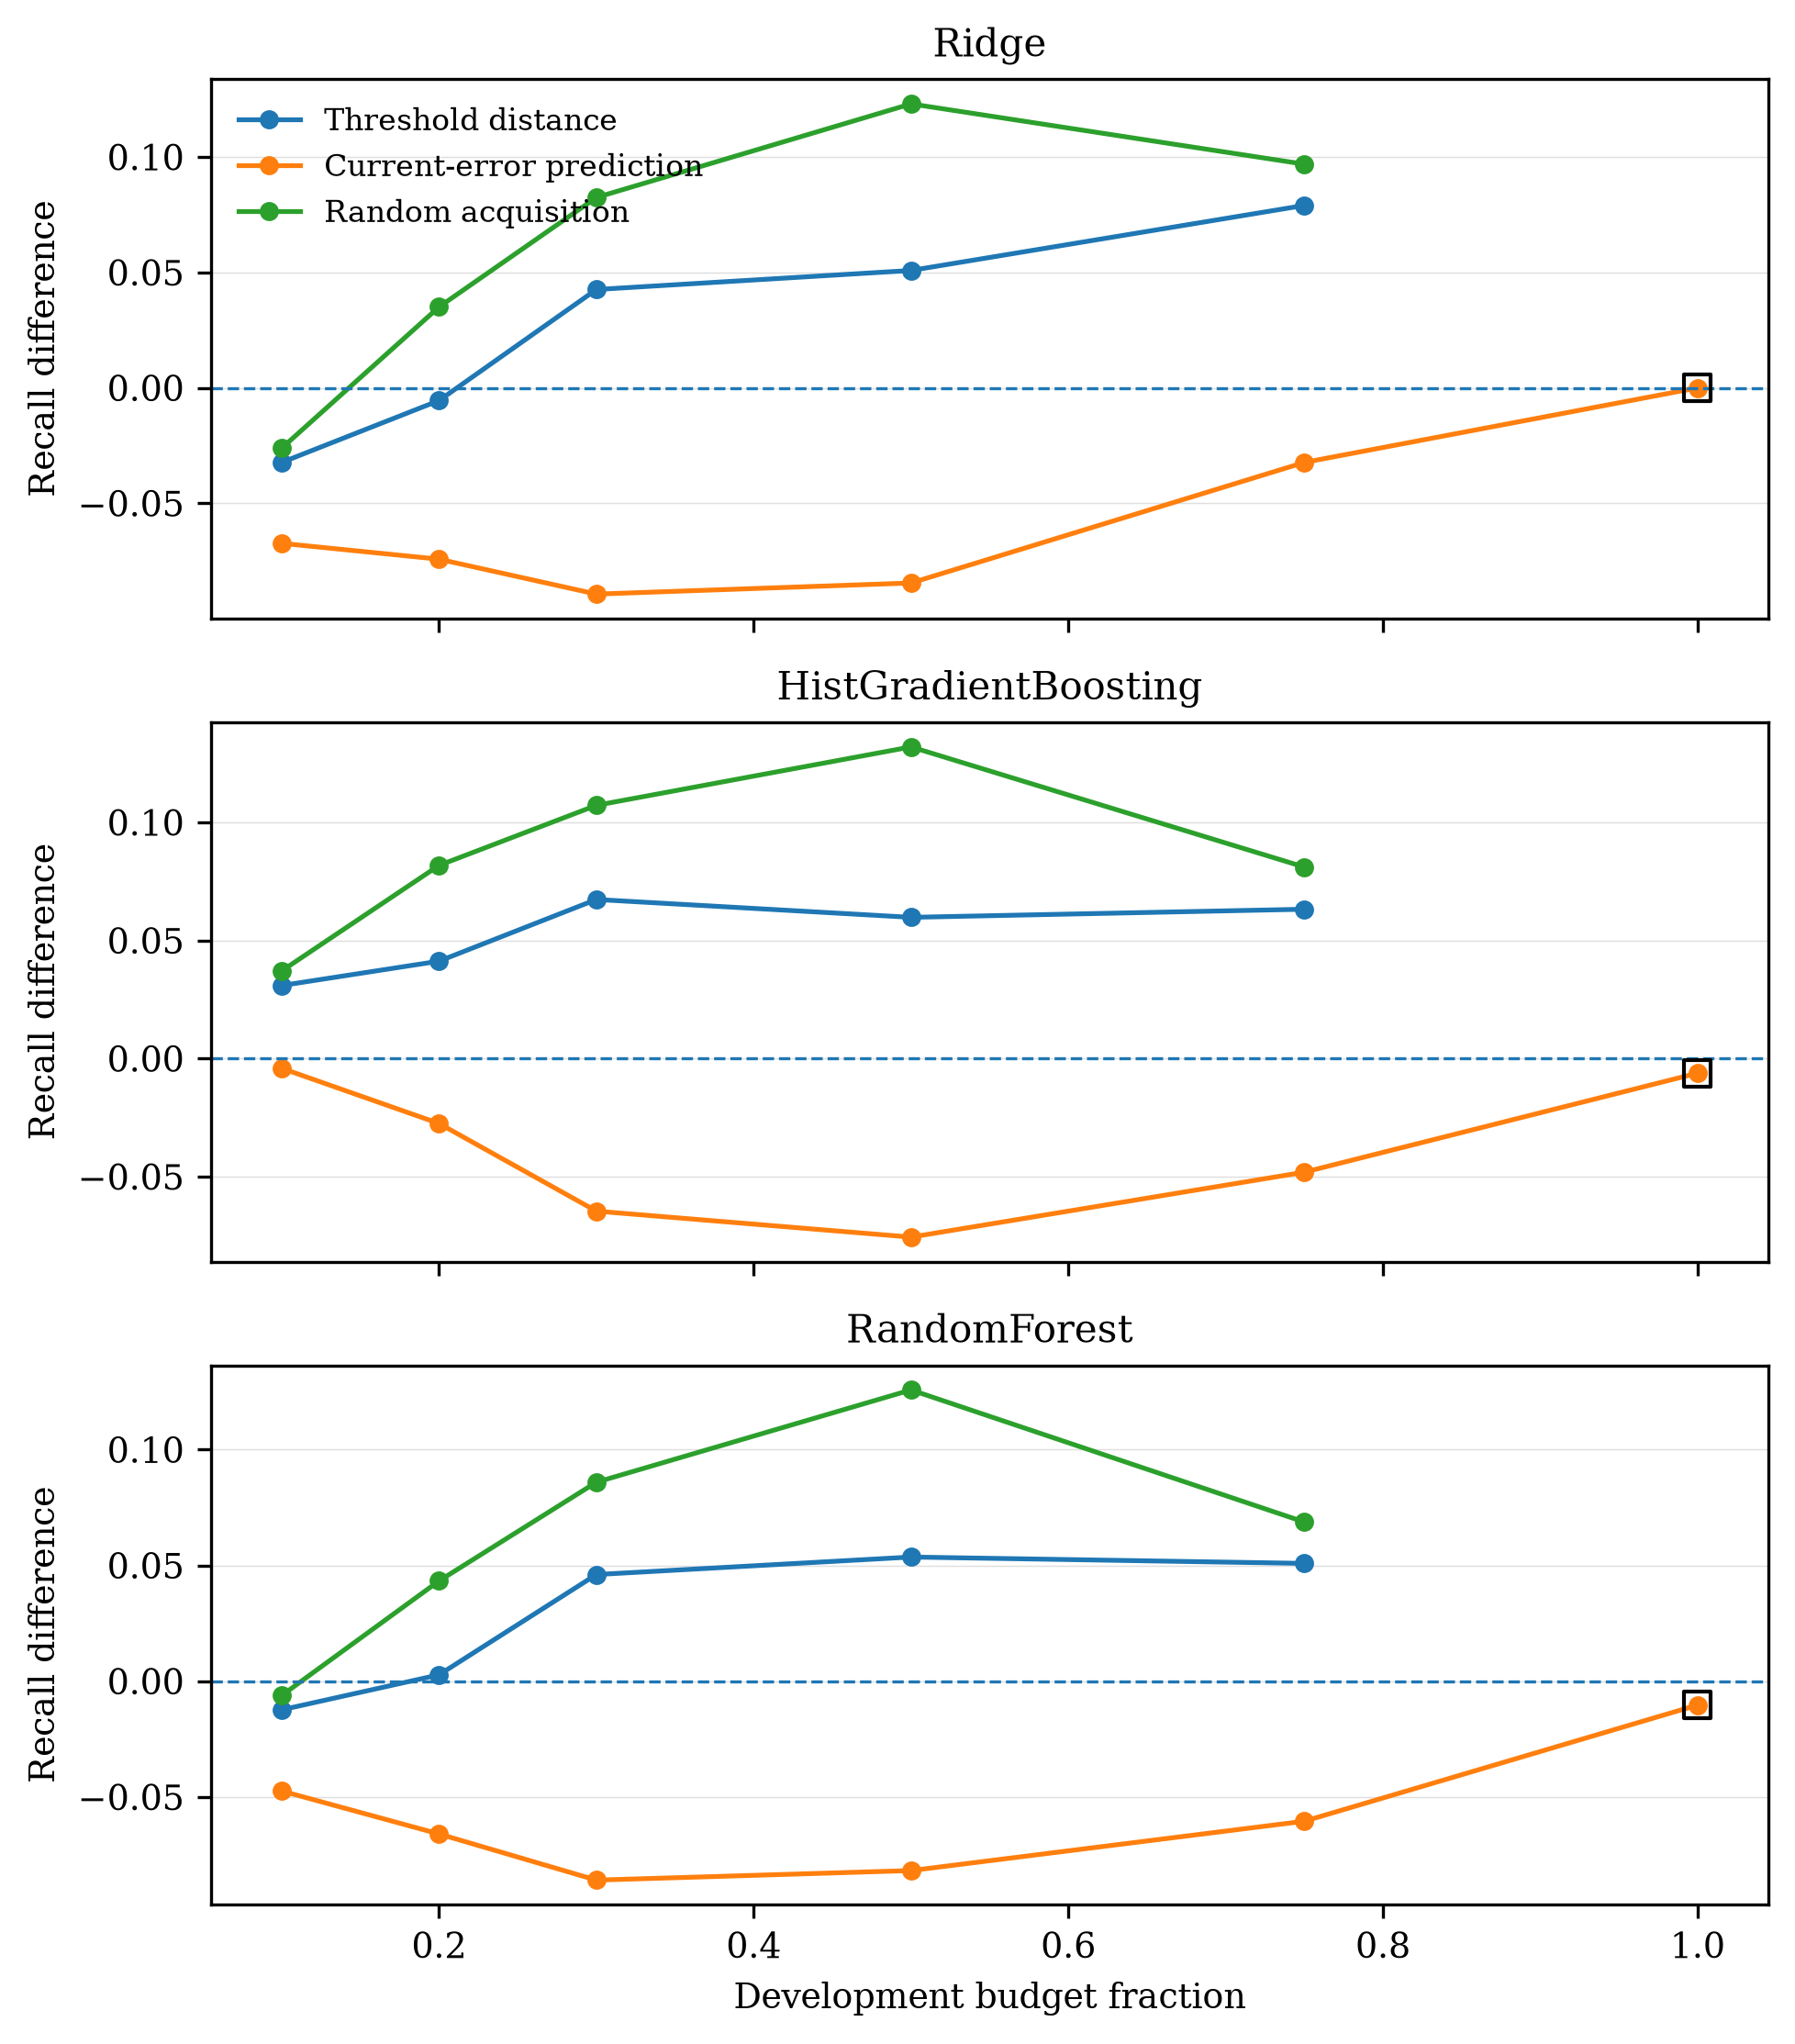
\includegraphics[
    width=0.96\linewidth
]{
    figures/development_recall_differences.png
}
\caption{
Mean development recall difference between each signed-value
family and the primary selective comparators. Positive values alone
do not establish improvement; recall comparison is admissible only
after paired cost equivalence. Square outlines denote
cost-equivalence passes.
}
\label{fig:recall}
\end{figure}

Figure~\ref{fig:equiv} makes the principal failure mode explicit:
the cost-equivalence pass rate is \(1/16\) for every signed-value
family.

\begin{figure}[H]
\centering
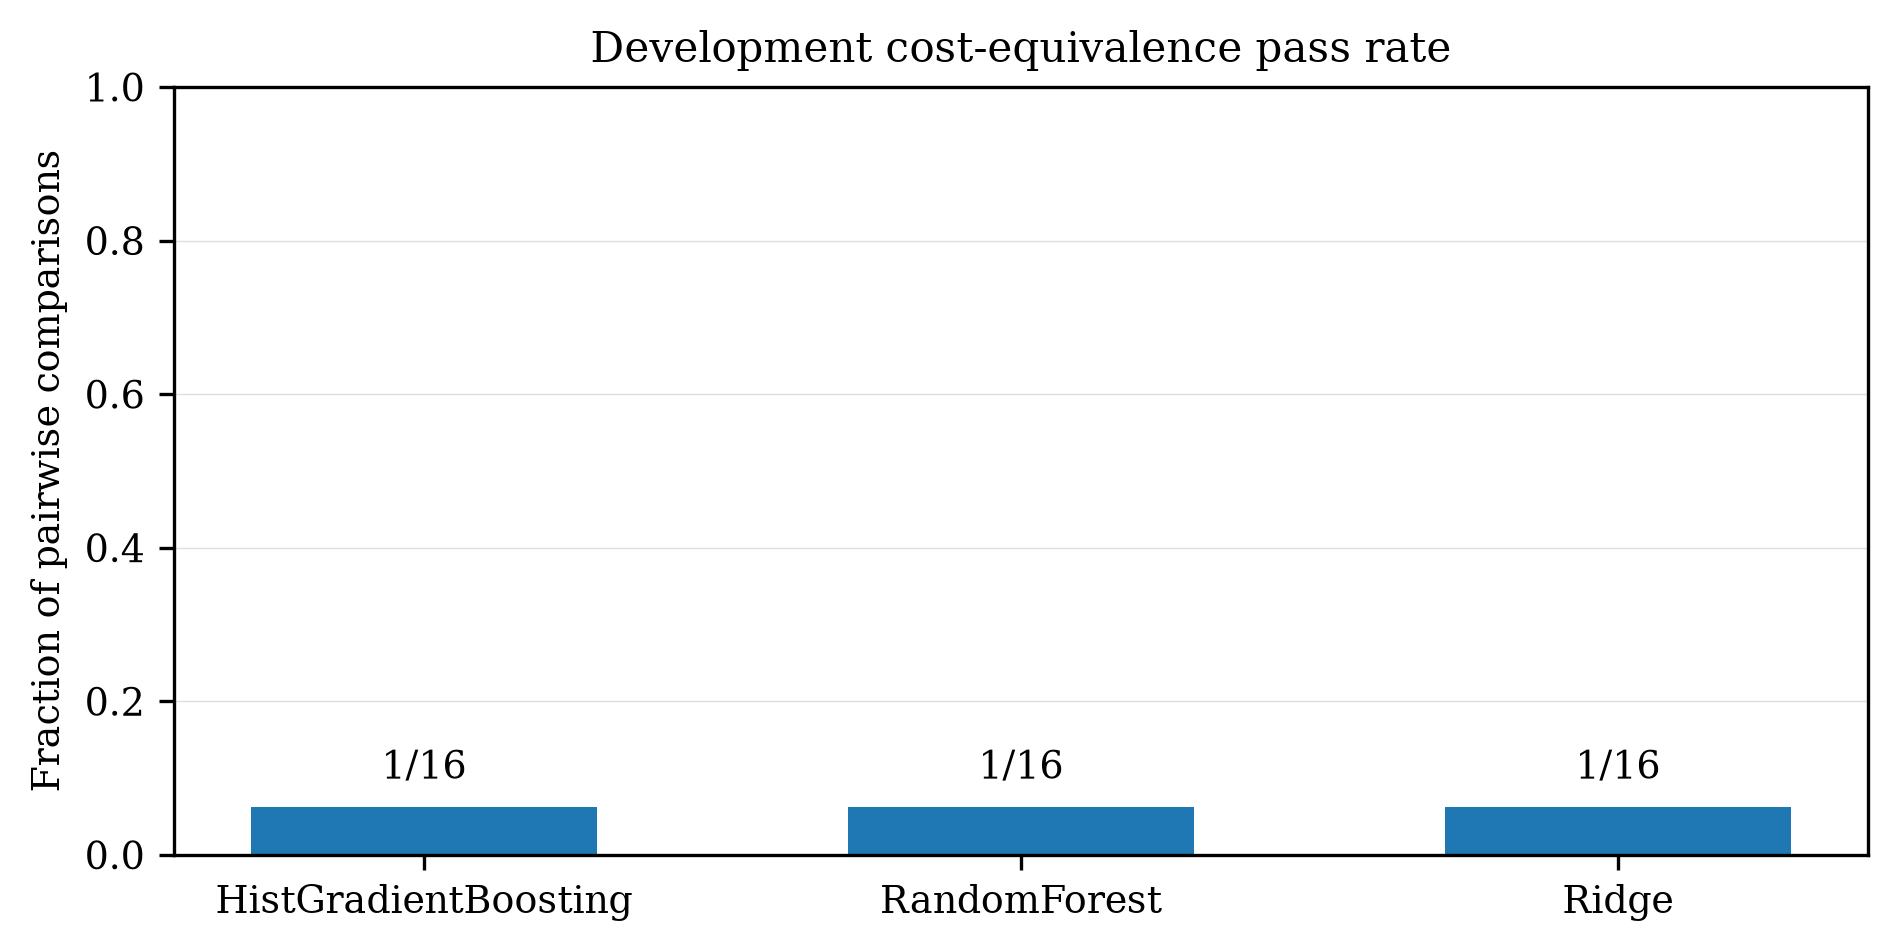
\includegraphics[
    width=0.80\linewidth
]{
    figures/cost_equivalence_pass_rate.png
}
\caption{
Fraction of primary development comparisons passing the paired
cost-equivalence test. All three signed-value model families pass
one of sixteen comparisons.
}
\label{fig:equiv}
\end{figure}

\subsection{Reference endpoints}

Table~\ref{tab:endpoints} reports the reference endpoints averaged
across the five fold seeds. Never acquisition has mean recall
\BaseRecall{} and mean FPR \BaseFPR{}. Always acquisition increases
mean recall to \AlwaysRecall{} at an average component total of
\AlwaysComponentCost{} ms. Direct-fusion models operate at
approximately the full acquisition cost and are therefore reported
as full-cost endpoints rather than selective same-cost comparators.

\begin{table}[t]
\centering
\scriptsize
\caption{
Development endpoint metrics averaged across five fold seeds.
Costs are measured component totals. FPR values are descriptive
development measurements, not finite-sample risk certificates.
}
\label{tab:endpoints}
\resizebox{\textwidth}{!}{
\begin{tabular}{
    ll
    r
    r
    r
    r
}
\toprule
Endpoint &
Family &
Mean cost (ms) &
Recall &
Mean FPR &
Maximum seed FPR \\
\midrule
never acquire & base policy & 43.78 & 0.2179 & 0.0504 & 0.0516 \\
always acquire & augmented policy & 3,746.4 & 0.8570 & 0.0470 & 0.0494 \\
direct fusion & HistGradientBoosting & 3,746.5 & 0.8667 & 0.0490 & 0.0509 \\
direct fusion & Logistic regression & 3,743.9 & 0.8598 & 0.0473 & 0.0494 \\
direct fusion & RandomForest & 3,781.9 & 0.8577 & 0.0491 & 0.0509 \\

\bottomrule
\end{tabular}
}
\end{table}

The base endpoint itself has maximum seed FPR
\BaseMaxFPR{}, slightly above 0.05. Some direct-fusion models also
cross 0.05 in at least one seed. These observations reinforce the
distinction between development point estimates and formal risk
control.

\subsection{Latency heterogeneity and upper-tail cost}

The optional monitor dominates runtime. Its measured mean is
\OptionalMean{} ms, median \OptionalMedian{} ms, p95
\OptionalPninetyfive{} ms, p99 \OptionalPninetynine{} ms, and
maximum \OptionalMaximum{} ms. By comparison, the mean base-monitor
stage is \BaseMonitorMean{} ms and the complete-text embedding stage
averages \EmbeddingMean{} ms.

Router inference is comparatively inexpensive for Ridge
(\RidgeRouterMean{} ms) and HistGradientBoosting
(\HGBRRouterMean{} ms), while the RandomForest signed-value router
is materially heavier at \RFRouterMean{} ms. These differences are
small relative to optional-monitor execution but remain part of the
online acquisition cost.

\begin{figure}[H]
\centering
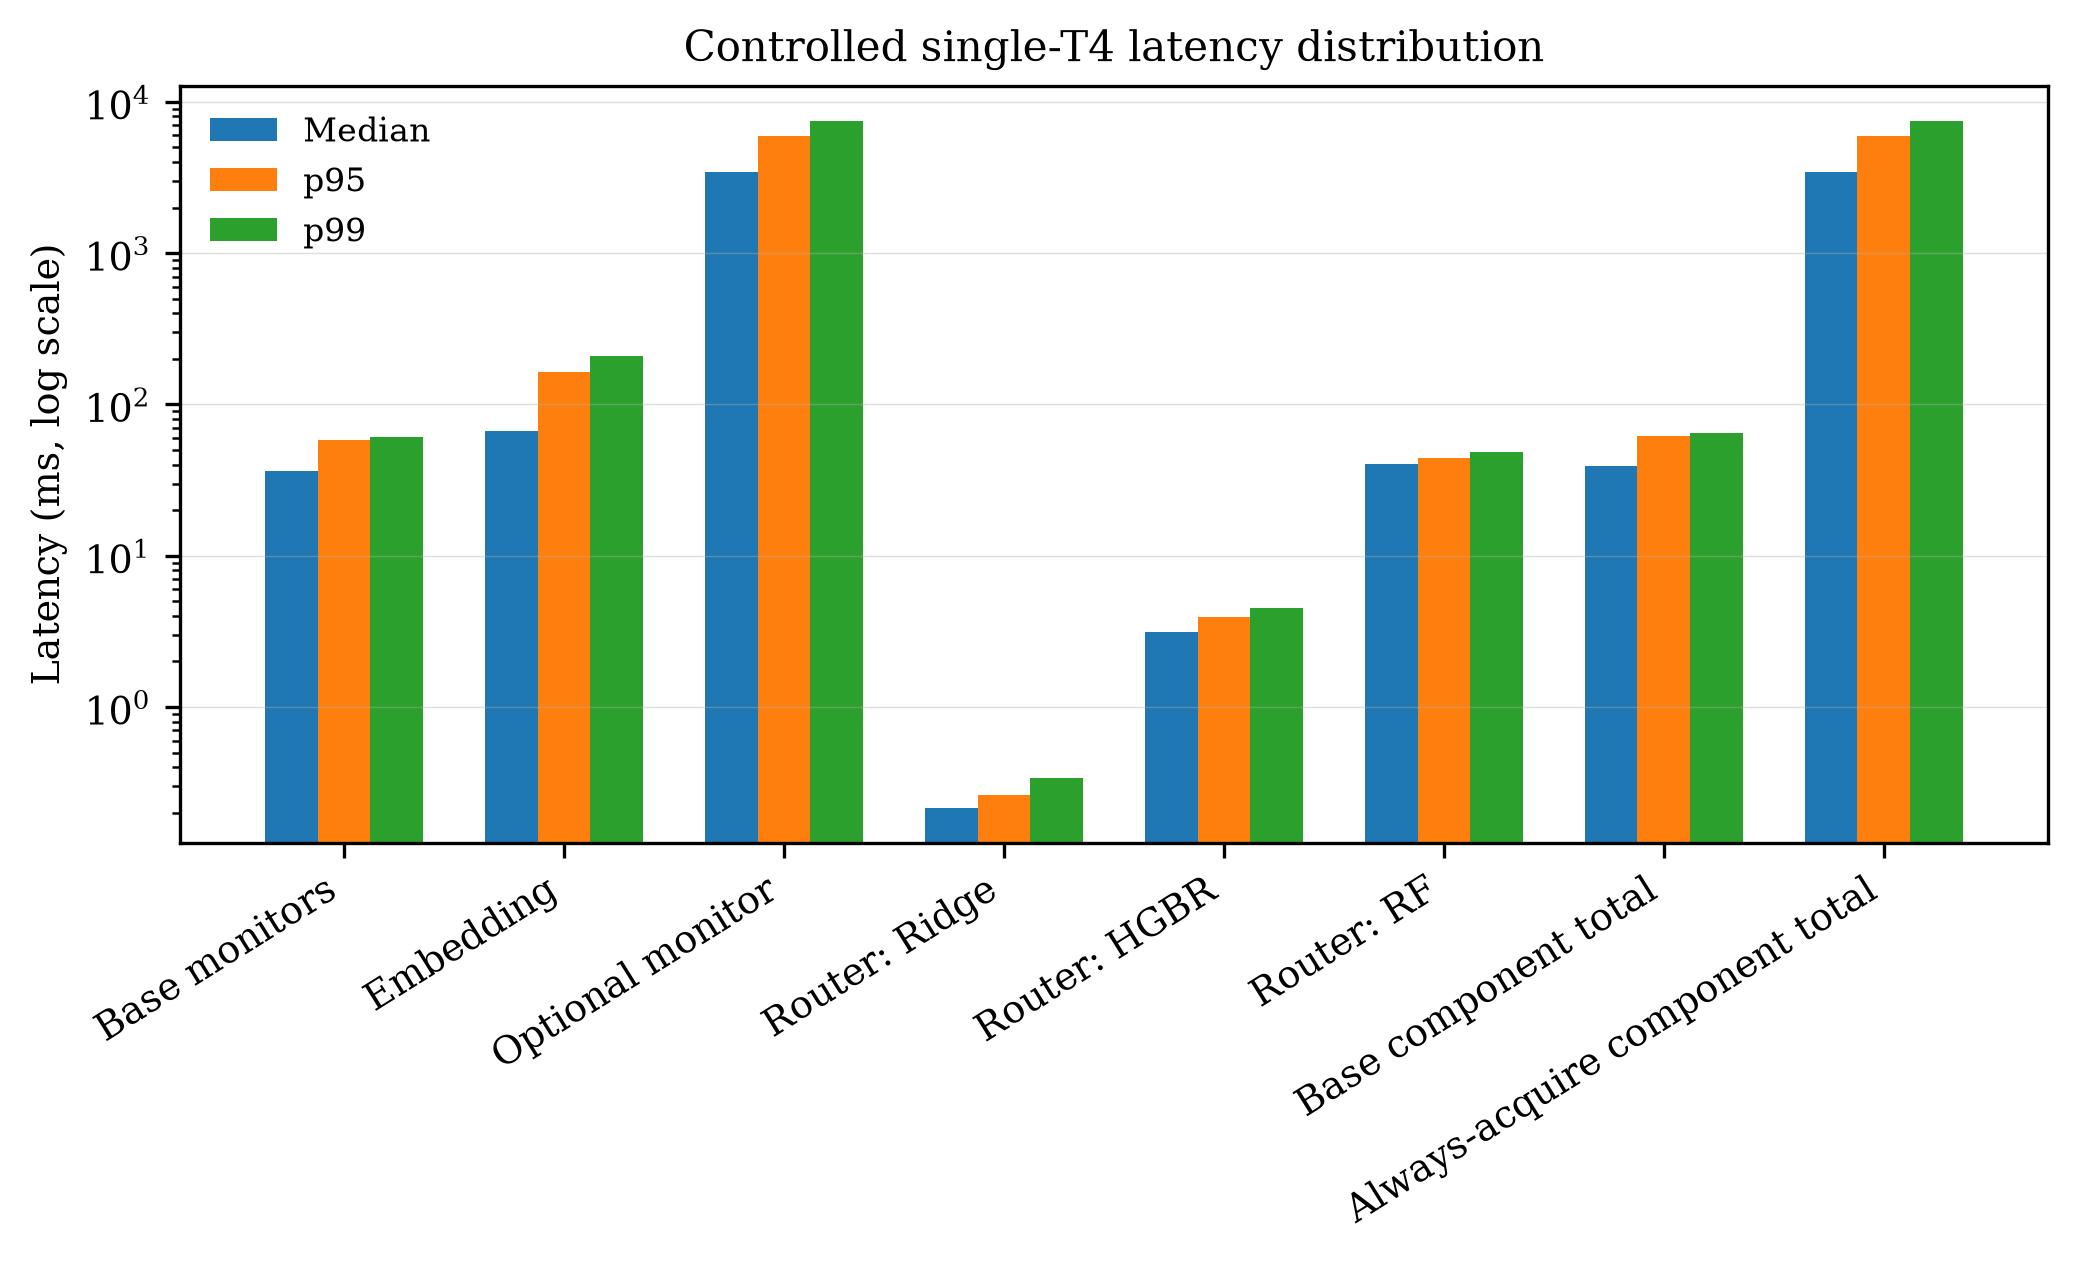
\includegraphics[
    width=0.96\linewidth
]{
    figures/controlled_t4_latency_tails.png
}
\caption{
Controlled single-T4 latency distributions. Bars show median, p95,
and p99 latency. The logarithmic scale exposes the separation
between router inference and optional-monitor execution. Component
totals are sums of directly timed non-overlapping stages.
}
\label{fig:latency}
\end{figure}

\begin{table}[t]
\centering
\tiny
\caption{
Controlled single-T4 latency summary in milliseconds. Tail
confidence intervals use 2,000 effective-group bootstrap resamples.
}
\label{tab:latency}
\resizebox{\textwidth}{!}{
\begin{tabular}{
    l
    r
    r
    r
    r
    c
    r
    c
    r
}
\toprule
Stage &
\(n\) &
Mean &
Median &
p95 &
95\% CI p95 &
p99 &
95\% CI p99 &
Maximum \\
\midrule
Base monitors & 1687 & 40.71 & 36.08 & 58.45 & [58.18, 58.84] & 61.12 & [60.84, 62.40] & 75.22 \\
Embedding & 1687 & 77.27 & 66.98 & 162.7 & [158.7, 166.9] & 209.1 & [202.5, 240.3] & 440.4 \\
Optional monitor & 1687 & 3,702.8 & 3,423.3 & 5,911.7 & [5,655.7, 5,960.9] & 7,456.4 & [6,856.7, 8,025.7] & 22,809.5 \\
Ridge router inference & 8435 & 0.219 & 0.214 & 0.261 & [0.259, 0.263] & 0.340 & [0.320, 0.361] & 0.554 \\
HGBR router inference & 8435 & 3.277 & 3.111 & 3.932 & [3.911, 3.954] & 4.516 & [4.402, 4.760] & 11.69 \\
RF router inference & 8435 & 40.95 & 40.59 & 44.25 & [43.98, 44.51] & 48.40 & [47.54, 49.64] & 82.02 \\
Base component total & 8435 & 43.78 & 39.21 & 61.60 & [61.23, 62.02] & 64.35 & [63.92, 65.61] & 78.64 \\
Always-acquire component total & 8435 & 3,746.4 & 3,462.7 & 5,975.6 & [5,716.8, 6,023.1] & 7,522.4 & [6,936.5, 8,104.6] & 22,887.9 \\

\bottomrule
\end{tabular}
}
\end{table}

No reported stage timed out in the controlled run. The absence of
timeouts does not make the latency distribution homogeneous:
optional-monitor p99 remains substantially above its median.

\section{Discussion}

The central result is methodological rather than a new routing
claim. Predictive performance of a routing score is not sufficient
to establish a better cascade. The policy must also survive
comparison at matched realized cost, under a threshold that can
actually be used online, with repeated grouped uncertainty and a
risk-control procedure that is independent of the evaluation set.

This distinction changes the interpretation of the earlier
development frontier. The historical frontier showed that ranked
development examples could produce favorable local recall under a
cost ceiling. Under the stricter protocol, that evidence is not
valid for router superiority because the comparator costs were not
matched by the present exact-cost criterion, random acquisition was
not represented by one jointly feasible frozen policy, FPR was
screened descriptively, and evaluation ranks participated in the
routing rule. The historical result remains useful as an example of
why an apparently favorable frontier can disappear under a more
deployment-valid comparison.

The signed-value correction is also substantive. Acquisition value
belongs to the pair of fitted policies. If the optional monitor can
change a correct base decision into an incorrect augmented decision,
then value is negative for that example. A nonnegative intrinsic
``monitor value'' therefore does not describe the deployed cascade.

The development no-go should not be interpreted as evidence that
selective acquisition is impossible in general. It establishes the
narrower and more defensible statement that the tested signed-value
families do not provide a selectable policy under this frozen
development comparison. Any renewed router study would require new
data and a newly justified protocol rather than post-hoc adjustment
to these development outcomes.

\section{Limitations}

The study intentionally leaves several claim gates unresolved.

First, final absolute budgets require fresh calibration. The
development analysis therefore uses measured component-cost anchors
only for preselection. These anchors cannot be reported as final
deployment exact-cost certificates.

Second, no signed-value family survives development selection.
Consequently there is no scientifically justified selected router
for a direct policy-level wall-clock end-to-end benchmark. The
latency evidence reported here consists of controlled per-stage
measurements and component totals, with full tail summaries.

Third, independent fresh calibration data were unavailable, so the
joint FPR-and-cost Learn Then Test certificate was not executed.

Fourth, fresh confirmatory data satisfying source separation, time
separation, deduplication, and the prespecified multi-rater labeling
requirements were unavailable. No confirmatory FPR upper bound,
Holm-adjusted recall comparison, or one-shot router-superiority
claim is therefore reported.

Finally, the existing protected legacy final and shift partitions
remain sealed in v2. Their reuse would not supply the fresh evidence
required by the protocol.

\section{Conclusion}

A stricter evaluation of the proposed safety-monitor router does
not support a routing-performance claim. Across five repeated
grouped seeds and three signed-value model families, no family has
a jointly feasible development operating point, and each family
passes only one of sixteen primary pairwise cost-equivalence tests.
Positive raw recall differences at some operating points therefore
cannot be converted into same-cost superiority claims.

The supported contribution is an evaluation and measurement
methodology for safety-monitor cascades: define policy-specific
signed value, use only pre-acquisition routing information, compare
selective policies at the same realized cost, require cost
equivalence before recall comparison, separate optimization from
risk certification, measure heterogeneous and upper-tail latency,
and reserve superiority claims for fresh confirmatory evidence.
Under those requirements, the present router remains a no-go.

\begin{thebibliography}{9}

\bibitem{clopper1934}
C. J. Clopper and E. S. Pearson,
``The use of confidence or fiducial limits illustrated in the
case of the binomial,''
\textit{Biometrika},
vol. 26, no. 4, pp. 404--413, 1934.


\bibitem{angelopoulos2025}
A. N. Angelopoulos, S. Bates, E. J. Cand\`es,
M. I. Jordan, and L. Lei,
``Learn then Test: Calibrating Predictive Algorithms to Achieve
Risk Control,''
\textit{The Annals of Applied Statistics},
vol. 19, no. 2, pp. 1641--1662, 2025.

\bibitem{hoeffding1963}
W. Hoeffding,
``Probability inequalities for sums of bounded random variables,''
\textit{Journal of the American Statistical Association},
vol. 58, no. 301, pp. 13--30, 1963.

\bibitem{bentkus2004}
V. Bentkus,
``On Hoeffding's inequalities,''
\textit{The Annals of Probability},
vol. 32, no. 2, pp. 1650--1673, 2004.

\bibitem{efron1979}
B. Efron,
``Bootstrap methods: Another look at the jackknife,''
\textit{The Annals of Statistics},
vol. 7, no. 1, pp. 1--26, 1979.

\bibitem{holm1979}
S. Holm,
``A simple sequentially rejective multiple test procedure,''
\textit{Scandinavian Journal of Statistics},
vol. 6, no. 2, pp. 65--70, 1979.

\end{thebibliography}

\end{document}
